\chapter{\IfLanguageName{dutch}{Frontend}{Frontend}}
\label{ch:frontend}

\section{\IfLanguageName{dutch}{Ontwikkeling}{Development}}
Zoals verteld in hoofdstuk \ref{ch:backend} is er gebruik gemaakt van de MEVN stack. Dit wilt zeggen dat de webapplicatie ontwikkeld is in Vue, een nieuwer javascript-framework. De code van deze webapplicatie is opensource en staat online op \href{https://github.com/IndyVC/bap-frontend}{een github repository}.
\newline
Voor de webapplicatie (zie figuur: \ref{fig:webapplicatie}) is er gebruik gemaakt van 'google maps'. Google maps is een veelgebruikte technologie waardoor dezelfde layout een vorm van betrouwbaarheid en herkenbaarheid geeft. Hierdoor voelt de webapplicatie gemakkelijk aan om te gebruiken. Naast het tracken zelf, weergeeft het ook extra informatie, zoals welke methode gebruikt wordt (zie hoofdstuk \ref{ch:backend}), hoe snel de GPS-tracker zich voort beweegt en hoe betrouwbaar de coördinaten zijn (aantal satellieten). De gebruiker is instaat om de geschiedenis van lokaties te verwijderen aan de hand van een knop.
\newline
Voor de implementatie van google maps is er gebruik gemaakt van een opensource en gratis te gebruiken library, namelijk \href{https://www.npmjs.com/package/vue2-google-maps}{vue2-google-maps}.
\begin{figure}
	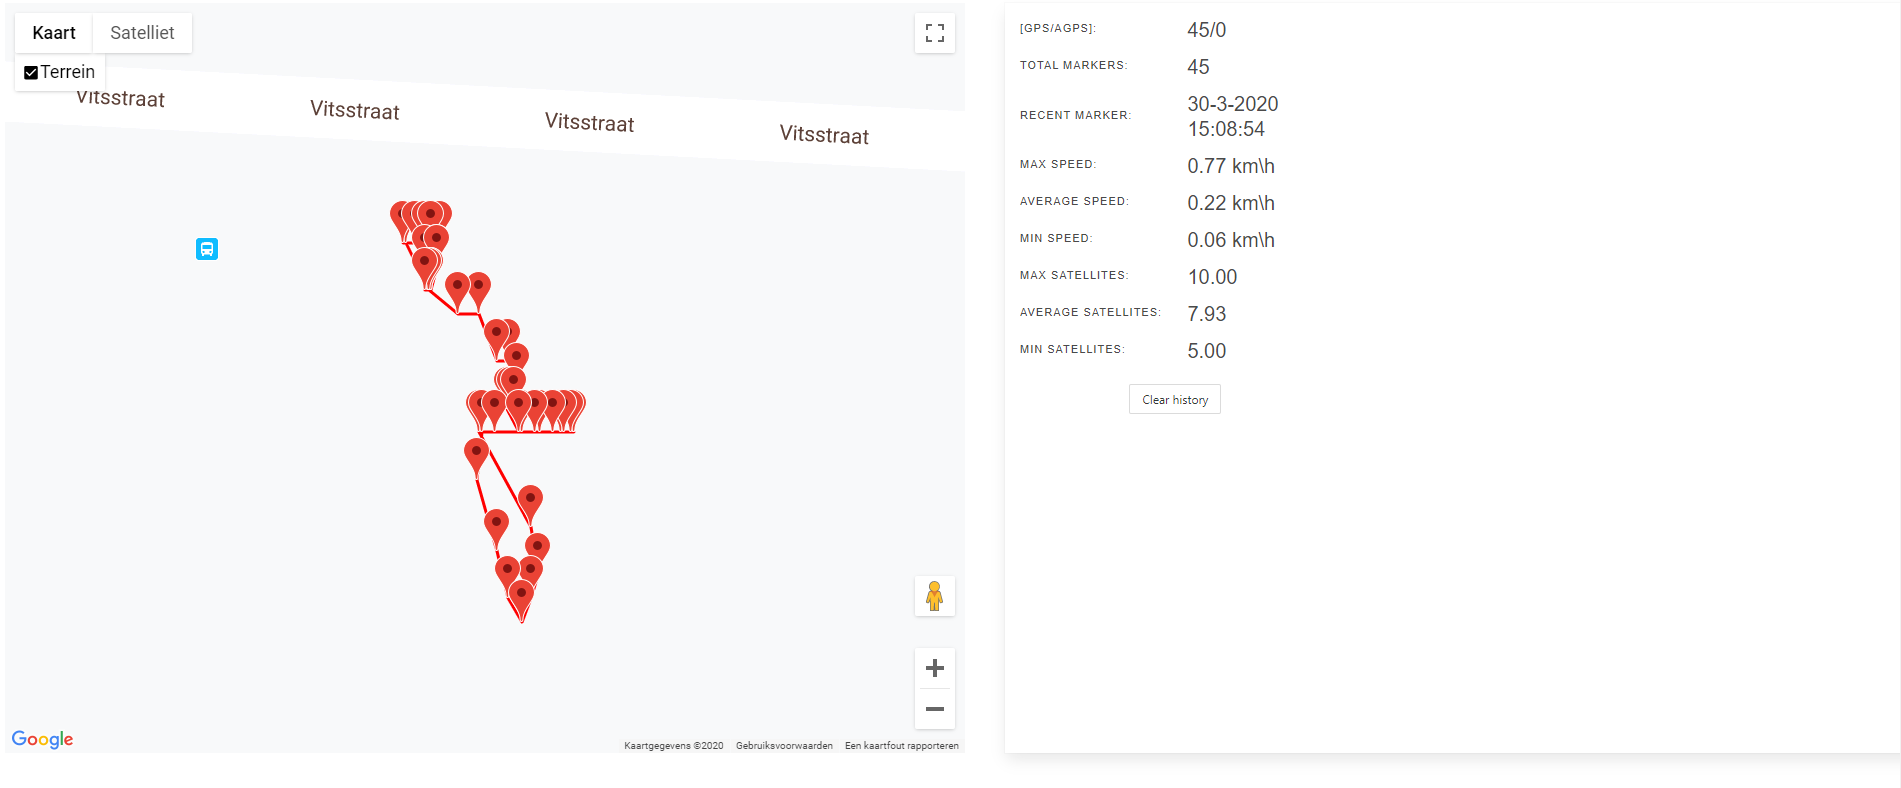
\includegraphics[width=\textwidth,height=\textheight,keepaspectratio]{webapplicatie.png}
	\caption{Webapplicatie}
	\label{fig:webapplicatie}
\end{figure}

\section{\IfLanguageName{dutch}{Deployment}{Deployment}}
Voor de website online te zetten is er gebruik gemaakt van netlify. \href{https://www.netlify.com/}{Netlify} is een hosting bedrijf dat een gratis plan aanbiedt. De webapplicatie staat \href{https://indy-bap-frontend.netlify.com/}{\underline{hier}} online.